\section{Third Member}

\subsection{Comments about the module}
The best parts of the module were the team activities as they were really fun especially when not assessed! Max Wilson was great, handled the feedback well and his lecture style was really good in explaining all the intricacies of the module.

\subsection{Selfie with Max}

\begin{figure}[h!]
\caption{Selfie with Max}
\centering
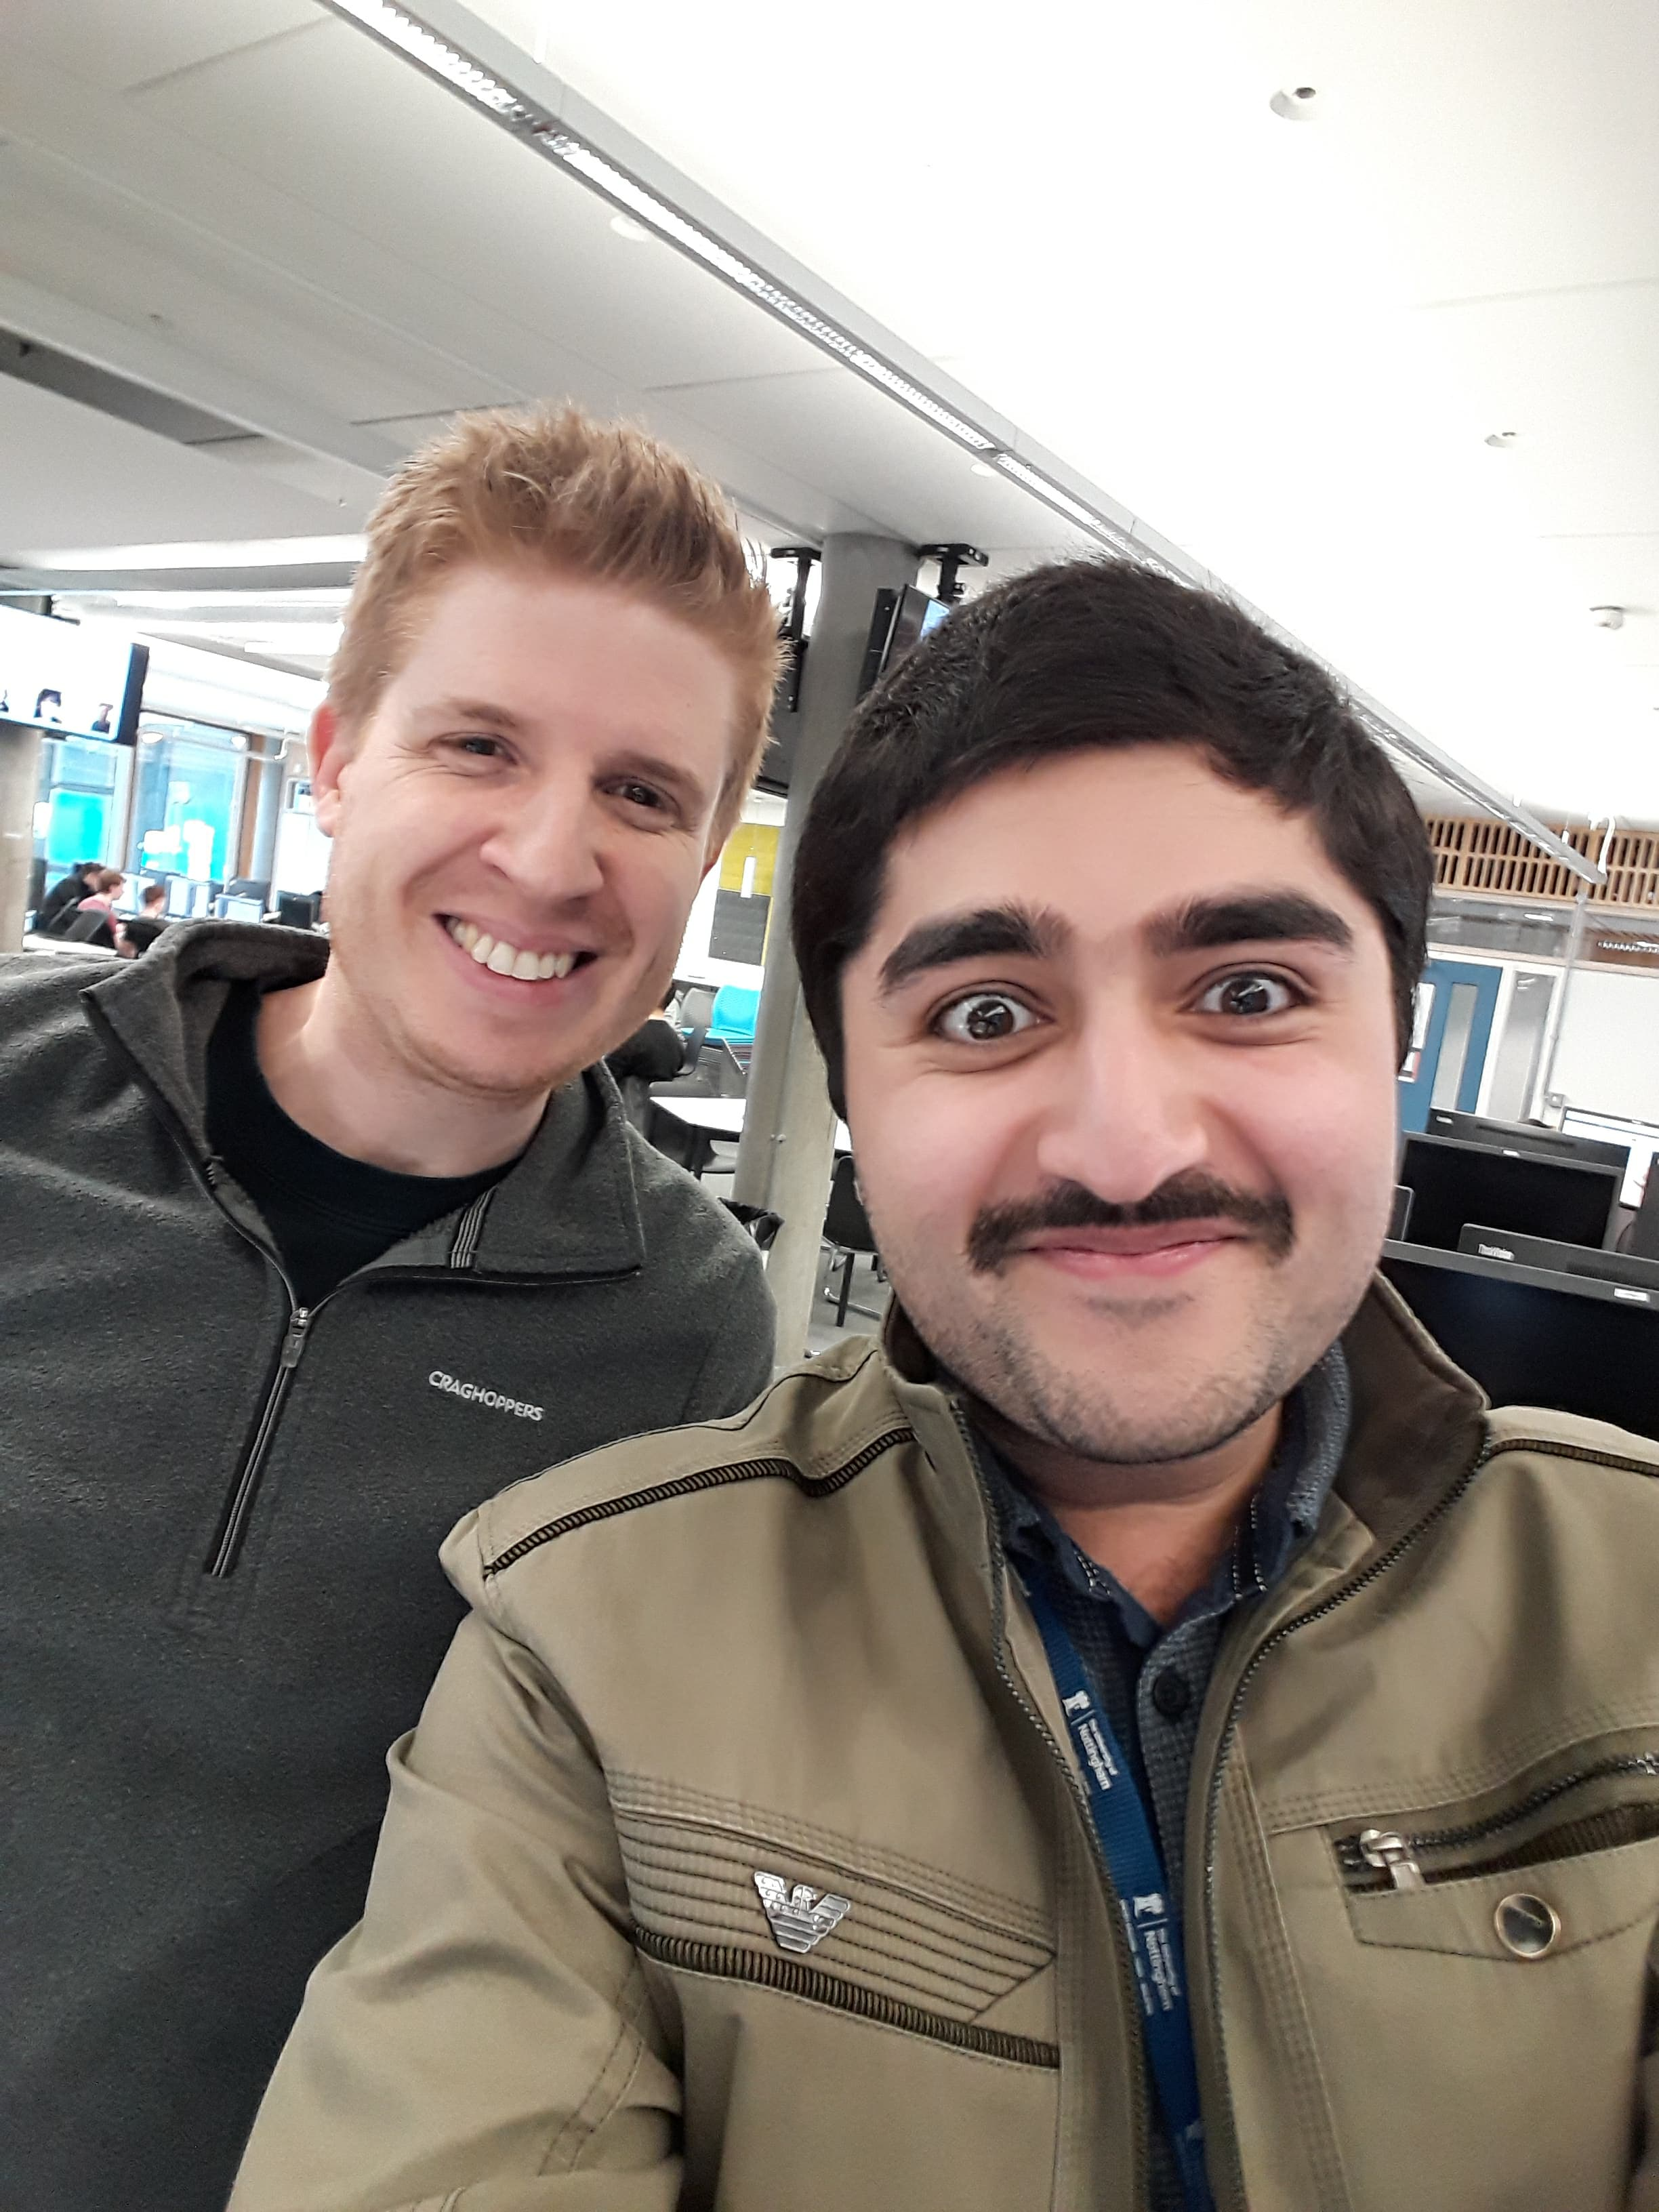
\includegraphics[width=0.5\textwidth]{Selfie_with_max.jpg}
\label{fig:selfie}
\end{figure}

You can then use the label of the figure to reference it later with the command ${\backslash}ref$. you can comment out the next line to see an example of how it works.

My selfie with Max is in  Figure~\ref{fig:selfie}.

\subsection{What I have learned in this module}
I learnt about the software engineering process and how the requirement gathering is the most important part of the whole thing. There are several different methods to developing the software the most favoured one is agile development however it doesn't produce documents that the manager requires. I also learnt about the various methods in collecting information and presenting it.

